%%%%%%%%%%%%%%%%%%%%%%%%%%%%%%%%%%%%%%%%%%%%%%%%%%%%%%%%%%%%%%%%%%%%%%%%%%%
%% This file is part of the book
%%
%% Algorithmic Graph Theory
%% http://code.google.com/p/graph-theory-algorithms-book/
%%
%% Copyright (C) 2009, 2010, 2011 Minh Van Nguyen <nguyenminh2@gmail.com>
%%
%% See the file COPYING for copying conditions.
%%%%%%%%%%%%%%%%%%%%%%%%%%%%%%%%%%%%%%%%%%%%%%%%%%%%%%%%%%%%%%%%%%%%%%%%%%%

%% digraph
\subfigure[]{
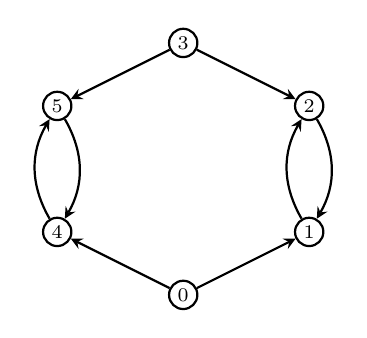
\begin{tikzpicture}
[arrowDecorate/.style={->,>=stealth,thick},%
  nodeDecorate/.style={shape=circle,inner sep=1.5pt,draw,thick},%
  scale=0.8]
\scriptsize
%% nodes or vertices
\foreach \nodename/\x/\y in {1/2/1, 2/2/3, 3/0/4, 0/0/0, 4/-2/1, 5/-2/3}
{
  \node (\nodename) at (\x,\y) [nodeDecorate] {$\nodename$};
}
%% edges or lines
\path
(1) edge[arrowDecorate,bend left] node {} (2)
(2) edge[arrowDecorate,bend left] node {} (1)
(3) edge[arrowDecorate] node {} (2)
(3) edge[arrowDecorate] node {} (5)
(0) edge[arrowDecorate] node {} (1)
(0) edge[arrowDecorate] node {} (4)
(4) edge[arrowDecorate,bend left] node {} (5)
(5) edge[arrowDecorate,bend left] node {} (4);
\end{tikzpicture}
%%
%%
\qquad\qquad
%%
%%
\begin{tikzpicture}
\node at (0,0) {%
$
\begin{bmatrix}
0      & 1      & 2      & \infty & 1      & 2 \\
\infty & 0      & 1      & \infty & \infty & \infty \\
\infty & 1      & 0      & \infty & \infty & \infty \\
\infty & 2      & 1      & 0      & 2      & 1 \\
\infty & \infty & \infty & \infty & 0      & 1 \\
\infty & \infty & \infty & \infty & 1      & 0
\end{bmatrix}
$
};
\end{tikzpicture}
}
%%
%%
\qquad
%% graph
\subfigure[]{
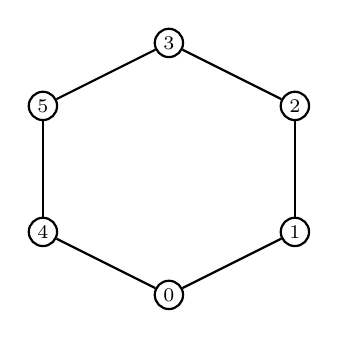
\begin{tikzpicture}
[lineDecorate/.style={-,thick},%
  nodeDecorate/.style={shape=circle,inner sep=1.5pt,draw,thick},%
  scale=0.8]
\scriptsize
%% nodes or vertices
\foreach \nodename/\x/\y in {1/2/1, 2/2/3, 3/0/4, 0/0/0, 4/-2/1, 5/-2/3}
{
  \node (\nodename) at (\x,\y) [nodeDecorate] {$\nodename$};
}
%% edges or lines
\path
\foreach \startnode/\endnode in {1/2, 1/0, 2/3, 3/5, 0/4, 4/5}
{
  (\startnode) edge[lineDecorate] node {} (\endnode)
};
\end{tikzpicture}
%%
%%
\qquad\qquad
%%
%%
\begin{tikzpicture}
\node at (0,0) {%
$
\begin{bmatrix}
0 & 1 & 2 & 3 & 1 & 2 \\
1 & 0 & 1 & 2 & 2 & 3 \\
2 & 1 & 0 & 1 & 3 & 2 \\
3 & 2 & 1 & 0 & 2 & 1 \\
1 & 2 & 3 & 2 & 0 & 1 \\
2 & 3 & 2 & 1 & 1 & 0
\end{bmatrix}
$
};
\end{tikzpicture}
}
